\chapter{Предварительная обработка изображений датасета}

После получения достаточного количества изображений для составления датасета необходимо провести их предварительную обработку и разметку. Это один из самыхважных этапов работы, поскольку от качества разметки напрямую зависит точность и эффективность последующей работы модели.

Для корректной работы модели YOLO требуется создать иерархическую структуру папок, в которой изображения и соответствующие метки будут разделены на тренировочную и валидационную выборки. Стандартная структура включает следующие директории:

\begin{enumerate}
    \item Директория train -- содержит тренировочную выборку:
    \begin{enumerate}
        \item images -- изображения;
        \item labels -- метки к изображениям.
    \end{enumerate}
    \item Директория val -- содержит валидационную выборку:
    \begin{enumerate}
        \item images -- изображения;
        \item labels -- метки к изображениям.
    \end{enumerate}
\end{enumerate}

Набор классов, пути к выборкам и параметры конфигурации задаются в YAML-файле, который передается при обучении модели. Содержимое такого файла для данной модели:

\begin{code}
\captionof{listing}{\label{code:train-captcha}Параметры конфигурации для обучения модели}
\vspace{-0.5cm}
{\small
\inputminted[mathescape,linenos,frame=lines,breaklines]{yaml}{code/train_captcha.yaml}
}
\end{code}
\vspace{-0.4cm}

Для создания меток используется инструмент CVAT (Computer Vision Annotation Tool) -- многофункциональное веб-приложение с поддержкой аннотации объектов с помощью полигонов, прямоугольников и других форм. CVAT позволяет экспортировать разметку напрямую в формат, совместимый с YOLO~\cite{CVAT}.

Поскольку CAPTCHA-изображения часто содержат объекты с нечёткими контурами, наложением и визуальными искажениями, особенно важно использовать ручную точную разметку, а не ограничиваться автоматическими методами. Выделение объектов должно проводиться как можно точнее, с учётом геометрии контуров. На рисунке ниже представлен пример изображения с размеченными объектами:

\begin{figure}[H]
    \centering
    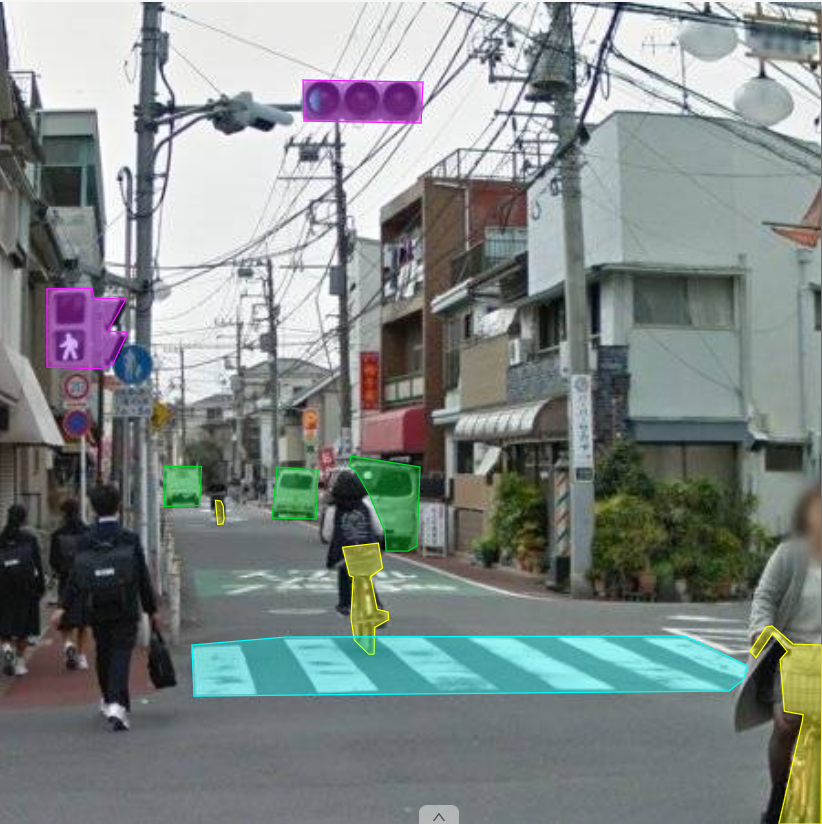
\includegraphics[width=0.9\linewidth]{imgs/captcha-poligons.png}
    \caption{Пример разметки изображения с тестовой CAPTCHA.}
    \label{fig:mask-captcha}
\end{figure}
\vspace{-0.5cm}

Кроме того, разметка позволяет учесть сразу несколько объектов разных классов на одном изображении, что особенно характерно для CAPTCHA, где в одной сетке могут одновременно находиться, например, автомобили и автобусы. Такой подход положительно влияет на обобщающую способность модели.

В случае, если количество данных по отдельным классам окажется недостаточным, можно дополнительно использовать методы аугментации: вращение, масштабирование, искажение цвета и контраста. Однако при хорошо организованном парсинге и разметке зачастую удается обойтись без аугментации.
